\documentclass{article}
\usepackage[utf8]{inputenc}

\usepackage{float}
\usepackage{subcaption}
\usepackage{bussproofs}
\usepackage[
style=alphabetic,
sorting=ynt
]{biblatex}
\usepackage{float}
\usepackage{quiver}
\usepackage{verbatim}
\usepackage{tikz}
\usepackage{circuitikz}

\addbibresource{main.bib}

\usepackage{amsmath}
\usepackage{amssymb}
\usepackage{graphicx}
\usepackage{prelude}
\usepackage{hyperref}
\usepackage{cleveref}

\hypersetup{
  colorlinks=true,
  linkcolor=red,
  citecolor=green
}

\renewcommand\qedsymbol{$\Box$}
\renewcommand*{\proofname}{\textcolor{ocre}{\textit{Proof.}}}
\renewcommand\labelitemi{-}

\binoppenalty=10000
\relpenalty=10000

\begin{document}
\begin{titlepage}
    \begin{center}

        
        \Large
        \textbf{ÉCOLE NORMALE SUPÉRIEURE PARIS-SACLAY}
        \vspace{0.3cm}
        \begin{figure}[h]
            \centering
            
\includegraphics[width=0.5\linewidth]{LOGOS_ENS.png}
        \end{figure}

        \vspace{3cm}

        Master's Internship Report 

        \vspace{1em}
            
        \Huge
        \textbf{Towards a Next-Generation Univalent \\Proof Assistant}

        \vspace{2.5cm}
            
        \LARGE
        \textbf{Raphaël Sterbac}

        Under the supervision of \textbf{Jon Sterling}

        (February - July 2026)
            
        \vfill
            
            
        \vspace{0.8cm}


        \begin{figure}[h]
            \centering
            
\includegraphics[width=0.4\linewidth]{cambridge-logo.jpg}
        \end{figure}
    \end{center}
\end{titlepage}

\begin{abstract}
    
\end{abstract}

\section{Introduction}

\section{A new algebraic Universe Hierarchy}

\subsection{The syntax} \label{rules}

In this section we define a new syntax for universe hierarchies, which aims at making them
more easy to work with on the engineering side. The main idea is to introduce a "smallness" judgement,
which correspond to the reflection of $\U_i$ in the $\Type$ world. The rules of this theory
$\cT_F$ are described in the following:

\vspace{1em}

\noindent
\begin{minipage}{0.3\linewidth}
\begin{prooftree}
\def\fCenter{\mbox{\ $\vdash$\ }}
\AxiomC{$\Gamma \vdash A : \U_i$}
\UnaryInfC{$\Gamma \vdash \decode{A}_i \; \Small_i$}
\end{prooftree}
\end{minipage}
\hfill
\begin{minipage}{0.3\linewidth}
\begin{prooftree}
\def\fCenter{\mbox{\ $\vdash$\ }}
\AxiomC{$\Gamma \vdash A : \Small_i$}
\UnaryInfC{$\Gamma \vdash \code{A}_i : \U_i$}
\end{prooftree}
\end{minipage}
\hfill
\begin{minipage}{0.3\linewidth}
\begin{prooftree}
\def\fCenter{\mbox{\ $\vdash$\ }}
\AxiomC{$\Gamma \vdash A : \U_i$}
\UnaryInfC{$\Gamma \vdash \decode{A}_i \; \Type$}
\end{prooftree}
\end{minipage}

\vspace{1em}

\noindent
\begin{minipage}{0.5\linewidth}
\begin{prooftree}
\def\fCenter{\mbox{\ $\vdash$\ }}
\AxiomC{$\Gamma \vdash A = B$}
\AxiomC{$\Gamma \vdash A \; \Small_i$}
\BinaryInfC{$\Gamma \vdash \code{A}_i = \code{B}_i : \U_i$}
\end{prooftree}
\end{minipage}
\hfill
\begin{minipage}{0.5\linewidth}
\begin{prooftree}
\def\fCenter{\mbox{\ $\vdash$\ }}
\AxiomC{$\Gamma \vdash A = B : U_i$}
\UnaryInfC{$\Gamma \vdash \decode{A}_i = \decode{B}_i$}
\end{prooftree}
\end{minipage}

\vspace{1em}

\noindent
\begin{minipage}{0.5\linewidth}
\begin{prooftree}
\def\fCenter{\mbox{\ $\vdash$\ }}
\AxiomC{$\Gamma \vdash A : \Small_i$}
\UnaryInfC{$\Gamma \vdash \decode{\code{A}_i}_i = A$}
\end{prooftree}
\end{minipage}
\hfill
\begin{minipage}{0.5\linewidth}
\begin{prooftree}
\def\fCenter{\mbox{\ $\vdash$\ }}
\AxiomC{$\Gamma \vdash \decode{A}_i = \decode{B}_i$}
\UnaryInfC{$\Gamma \vdash A = B : U_i$}
\end{prooftree}
\end{minipage}

\vspace{2em}

Then, we need a smallness rule corresponding to every type formation rule:

\vspace{2em}

\noindent
\begin{minipage}{0.3\linewidth}
\begin{prooftree}
\def\fCenter{\mbox{\ $\vdash$\ }}
\AxiomC{$\Gamma \vdash i+1 \leq j$}
\UnaryInfC{$\Gamma \vdash \U_i : \Small_j$}
\end{prooftree}
\end{minipage}
\hfill
\begin{minipage}{0.3\linewidth}
\begin{prooftree}
\def\fCenter{\mbox{\ $\vdash$\ }}
\AxiomC{$\Gamma \vdash A \; \Small_i$}
\AxiomC{$\Gamma.A \vdash B \; \Small_i$}
\BinaryInfC{$\Gamma \vdash \Pi(A,B) \; \Small_i$}
\end{prooftree}
\end{minipage}
\hfill
\begin{minipage}{0.3\linewidth}
\begin{prooftree}
\def\fCenter{\mbox{\ $\vdash$\ }}
\AxiomC{$\Gamma \vdash \overline{u} \; \Small_i$}
\UnaryInfC{$\Gamma \vdash \D(\overline{u}) \; \Small_i$}
\end{prooftree}
\end{minipage}

\vspace{1em}

\noindent
\begin{minipage}{0.5\linewidth}
\begin{prooftree}
\def\fCenter{\mbox{\ $\vdash$\ }}
\AxiomC{$\Gamma \vdash A \; \Small_i$}
\AxiomC{$\Gamma.A \vdash B \; \Small_i$}
\BinaryInfC{$\Gamma \vdash \Sigma(A,B) \; \Small_i$}
\end{prooftree}
\end{minipage}
\hfill
\begin{minipage}{0.5\linewidth}
\begin{prooftree}
\def\fCenter{\mbox{\ $\vdash$\ }}
\AxiomC{$\Gamma \vdash A \; \Small_i$}
\UnaryInfC{$\Gamma.(x: A) . (y:A) \vdash x =_A y \; \Small_i$}
\end{prooftree}
\end{minipage}

\vspace{2em}


\begin{figure}[h]
\centering

\tikzset{every picture/.style={line width=0.75pt}} %set default line width to 0.75pt        

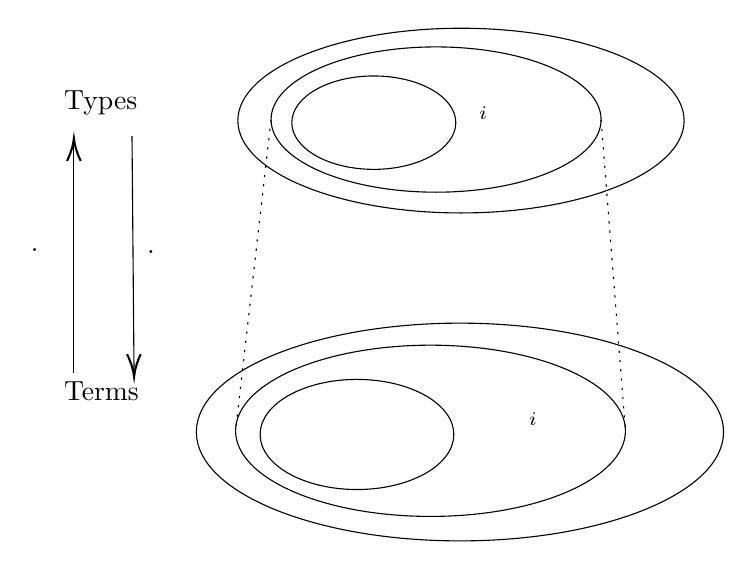
\begin{tikzpicture}[x=0.75pt,y=0.75pt,yscale=-1,xscale=1]
%uncomment if require: \path (0,300); %set diagram left start at 0, and has height of 300

%Shape: Ellipse [id:dp03901608556716085] 
\draw   (110,63.5) .. controls (110,38.92) and (158.13,19) .. (217.5,19) .. controls (276.87,19) and (325,38.92) .. (325,63.5) .. controls (325,88.08) and (276.87,108) .. (217.5,108) .. controls (158.13,108) and (110,88.08) .. (110,63.5) -- cycle ;
%Shape: Ellipse [id:dp09228997018809981] 
\draw   (126,63) .. controls (126,43.67) and (161.59,28) .. (205.5,28) .. controls (249.41,28) and (285,43.67) .. (285,63) .. controls (285,82.33) and (249.41,98) .. (205.5,98) .. controls (161.59,98) and (126,82.33) .. (126,63) -- cycle ;
%Shape: Ellipse [id:dp09230734801389129] 
\draw   (136,64.5) .. controls (136,52.07) and (153.68,42) .. (175.5,42) .. controls (197.32,42) and (215,52.07) .. (215,64.5) .. controls (215,76.93) and (197.32,87) .. (175.5,87) .. controls (153.68,87) and (136,76.93) .. (136,64.5) -- cycle ;
%Shape: Ellipse [id:dp7716542839814151] 
\draw   (90,213.54) .. controls (90,184.57) and (146.86,161.09) .. (217,161.09) .. controls (287.14,161.09) and (344,184.57) .. (344,213.54) .. controls (344,242.51) and (287.14,266) .. (217,266) .. controls (146.86,266) and (90,242.51) .. (90,213.54) -- cycle ;
%Shape: Ellipse [id:dp3664859998997495] 
\draw   (108.9,212.96) .. controls (108.9,190.17) and (150.95,171.7) .. (202.82,171.7) .. controls (254.69,171.7) and (296.74,190.17) .. (296.74,212.96) .. controls (296.74,235.74) and (254.69,254.21) .. (202.82,254.21) .. controls (150.95,254.21) and (108.9,235.74) .. (108.9,212.96) -- cycle ;
%Shape: Ellipse [id:dp7632685221556846] 
\draw   (120.72,214.72) .. controls (120.72,200.08) and (141.61,188.2) .. (167.38,188.2) .. controls (193.15,188.2) and (214.05,200.08) .. (214.05,214.72) .. controls (214.05,229.37) and (193.15,241.25) .. (167.38,241.25) .. controls (141.61,241.25) and (120.72,229.37) .. (120.72,214.72) -- cycle ;
%Straight Lines [id:da6719983041855007] 
\draw  [dash pattern={on 0.84pt off 2.51pt}]  (126,63) -- (108.9,212.96) ;
%Straight Lines [id:da34820569046037697] 
\draw  [dash pattern={on 0.84pt off 2.51pt}]  (285,63) -- (296.74,212.96) ;
%Straight Lines [id:da2671775247497892] 
\draw    (31,185) -- (31,118) -- (31,74) ;
\draw [shift={(31,72)}, rotate = 90] [color={rgb, 255:red, 0; green, 0; blue, 0 }  ][line width=0.75]    (10.93,-3.29) .. controls (6.95,-1.4) and (3.31,-0.3) .. (0,0) .. controls (3.31,0.3) and (6.95,1.4) .. (10.93,3.29)   ;
%Straight Lines [id:da9435994540795705] 
\draw    (59,71) -- (59.98,185) ;
\draw [shift={(60,187)}, rotate = 269.51] [color={rgb, 255:red, 0; green, 0; blue, 0 }  ][line width=0.75]    (10.93,-3.29) .. controls (6.95,-1.4) and (3.31,-0.3) .. (0,0) .. controls (3.31,0.3) and (6.95,1.4) .. (10.93,3.29)   ;

% Text Node
\draw (25,48) node [anchor=north west][inner sep=0.75pt]   [align=left] {{Types}};
% Text Node
\draw (25,188) node [anchor=north west][inner sep=0.75pt]   [align=left] {{Terms}};
% Text Node
\draw (9,124) node [anchor=north west][inner sep=0.75pt]   [align=left] {$\decode{.}$};
% Text Node
\draw (65,125) node [anchor=north west][inner sep=0.75pt]   [align=left] {$\code{.}$};
% Text Node
\draw (225,55.4) node [anchor=north west][inner sep=0.75pt]    {$\Small_{i}$};
% Text Node
\draw (248.94,203.18) node [anchor=north west][inner sep=0.75pt]    {$\U_{i}$};

\end{tikzpicture}
\caption{Our universe hierarchy and its reflection }
\end{figure}

The injectivity of the decoding function allows to axiomatise the judgements $\Small_i$
as propositions in our theory, not breaking the generalised algebraic character of the formulation.

\begin{definition}[Smallness judgement]
    When giving an algebraic formulation of our theory, we axiomatise the smallness judgement $\Small_i$
    as a proposition $\Small_i(A) : \Prop$.\\

    Hence, judgements $\Gamma \vdash A \; \Small_i$ will be a notation for $\Gamma \vdash p : \Small_i(A)$. 
    The notation is justified, and does not depend on $p$ because $\Small_i$ is a proposition.
\end{definition}

\begin{proposition}[Smallness is monotone]
    The following rule is derivable in $\cT_F$.
    
    \begin{prooftree}
    \def\fCenter{\mbox{\ $\vdash$\ }}
    \AxiomC{$\Gamma \vdash a  \; \Small_i$}
    \AxiomC{$\Gamma \vdash i < j$}
    \BinaryInfC{$\Gamma \vdash a  \; \Small_j$}
    \end{prooftree}
\end{proposition}

On top of that, we can define codes for the type connectives along with lifts, and prove
that they are directly coherent.

\begin{proposition}[Derivability of codes and lifts]\label{derivability}
    We can define the following codes for the type connectives.

    \begin{itemize}
        \item $t_i^j := \code{\decode{a}_i}_j$
        \item $\Pi^i := \code{\Pi(\decode{a}_i, \decode{b}_i)}$
        \item $\Sigma^i := \code{\Sigma(\decode{a}_i, \decode{b}_i)}$
        \item $\U_i^j := \code{U_i}$
    \end{itemize}

    Then, the following rules are derivable.

    \vspace{1em}

    \noindent
    \begin{minipage}{0.50\linewidth}
    \begin{prooftree}
    \def\fCenter{\mbox{\ $\vdash$\ }}
    \AxiomC{$\Gamma \vdash a: \U_n$}
    \AxiomC{$\Gamma,\decode{a}_n \vdash b: \U_n$}
    \BinaryInfC{$\Gamma \vdash \decode{\Pi^n \, a \, b}_n = \Pi(\decode{a}_n,\decode{b}_n)$}
    \end{prooftree}
    \end{minipage}
    \hfill
    \begin{minipage}{0.50\linewidth}
    \begin{prooftree}
    \def\fCenter{\mbox{\ $\vdash$\ }}
    \AxiomC{$\Gamma \vdash a: \U_n$}
    \AxiomC{$\Gamma,\decode{a}_n \vdash b: \U_n$}
    \AxiomC{$\Gamma \vdash n<p$}
    \TrinaryInfC{$\Gamma \vdash t_n^p(\Pi^n \, a \, b) = \Pi^p(t_n^p(a),t_n^p(b))$}
    \end{prooftree}
    \end{minipage}
    \vspace{1em}

    \noindent
    \begin{minipage}{0.50\linewidth}
    \begin{prooftree}
    \def\fCenter{\mbox{\ $\vdash$\ }}
    \AxiomC{}
    \UnaryInfC{$\Gamma \vdash \decode{\U_m^n}_n = \U_m$}
    \end{prooftree}
    \end{minipage}
    \hfill
    \begin{minipage}{0.50\linewidth}
    \begin{prooftree}
    \def\fCenter{\mbox{\ $\vdash$\ }}
    \AxiomC{$\Gamma \vdash n<m$}
    \UnaryInfC{$\Gamma \vdash t_n^p(\U_m^n) = \U_m^p : \U_p$}
    \end{prooftree}
    \end{minipage}
    \vspace{1em}

    \noindent
    \begin{minipage}{0.50\linewidth}
    \begin{prooftree}
    \def\fCenter{\mbox{\ $\vdash$\ }}
    \AxiomC{$\Gamma \vdash a : \U_m$}
    \AxiomC{$\Gamma \vdash n<m$}
    \BinaryInfC{$\Gamma \vdash \decode{t_m^n(a)}_n = \decode{a}_m$}
    \end{prooftree}
    \end{minipage}
    \hfill
    \begin{minipage}{0.50\linewidth}
    \begin{prooftree}
    \def\fCenter{\mbox{\ $\vdash$\ }}
    \AxiomC{$\Gamma \vdash a : \U_m$}
    \AxiomC{$\Gamma \vdash m<n<p$}
    \BinaryInfC{$\Gamma \vdash t_n^p(t_m^n(a)) = t_m^p(a): \U_p$}
    \end{prooftree}
    \end{minipage}
    \vspace{2em}
    
    \end{proposition}

\begin{proof}
    For example, $t_n^p(t_m^n(a)) = t_m^p(a)$ amounts at showing 
    $\code{\decode{\code{\decode{a}_m}_n}_n}_p = \code{\decode{a}_m}_p$, 
    and this can be derived as follows.

    \begin{prooftree}
    \def\fCenter{\mbox{\ $\vdash$\ }}
    \AxiomC{$\Gamma \vdash \decode{a}_m  \; \Small_m$}
    \AxiomC{$\Gamma \vdash m < n$}
    \BinaryInfC{$\Gamma \vdash \decode{a}_m  \; \Small_n$}
    \UnaryInfC{$\Gamma \vdash \decode{\code{\decode{a}_m}_n}_n = \decode{a}_m  \; \Type$}
    \AxiomC{$\Gamma \vdash \decode{a}_m  \; \Small_m$}
    \AxiomC{$\Gamma \vdash m < p$}
    \BinaryInfC{$\Gamma \vdash \decode{a}_m  \; \Small_p$}
    \BinaryInfC{$\Gamma \vdash \code{\decode{\code{\decode{a}_m}_n}_n}_p = \code{\decode{a}_m}_p : \U_p$}
    \end{prooftree}
\end{proof}

This shows that our system is at least as expressive as a theory with an usual Tarski universe
hierarchy. It is really interesting to note that the injectivity rule was not needed to prove
the derivability of all those rules. However, the injectivity will play a more intrinsic role
in providing that those lifts are canonical.\\

Semantically, we have the following situation

\begin{figure}[H]
\begin{subfigure}{0.5\textwidth}
% https://q.uiver.app/#q=WzAsNCxbMCwwLCJVXzAiXSxbMSwwLCJVXzEiXSxbMiwwLCIuLi4iXSxbMywwLCJUeXBlIl0sWzEsMl0sWzIsM10sWzEsMywiRWxfMSIsMSx7ImN1cnZlIjozfV0sWzAsMSwidF8wXjEiXSxbMCwzLCJFbF8wIiwyLHsibGFiZWxfcG9zaXRpb24iOjQwLCJvZmZzZXQiOjQsImN1cnZlIjo1fV1d
\[\begin{tikzcd}[sep=large]
    {\cU_0} & {\cU_1} & {...} & \cV
	\arrow["{t_0^1}", from=1-1, to=1-2]
	\arrow["{\El_0}"'{pos=0.4}, shift right=3, curve={height=30pt}, from=1-1, to=1-4]
	\arrow[from=1-2, to=1-3]
	\arrow["{\El_1}"{description}, curve={height=18pt}, from=1-2, to=1-4]
	\arrow[from=1-3, to=1-4]
\end{tikzcd}\]
\label{fig:subim1}
\end{subfigure}
\begin{subfigure}{0.5\textwidth}
% https://q.uiver.app/#q=WzAsNCxbMCwwLCJVXzAiXSxbMSwwLCJVXzEiXSxbMiwwLCIuLi4iXSxbMywwLCJUeXBlIl0sWzEsMl0sWzIsM10sWzAsMSwidF8wXjEiXSxbMywxLCIiLDEseyJvZmZzZXQiOjIsImN1cnZlIjotMywiY29sb3VyIjpbMCw2MCw2MF19XSxbMCwzLCIiLDEseyJvZmZzZXQiOjIsImN1cnZlIjo1LCJjb2xvdXIiOlswLDYwLDYwXX1dXQ==
\[\begin{tikzcd}[sep=large]
	{\cU_0} & {\cU_1} & {...} & \cV 
	\arrow["{t_0^1}", from=1-1, to=1-2]
	\arrow[shift right=3, color={rgb,255:red,214;green,92;blue,92}, curve={height=30pt}, from=1-1, to=1-4]
	\arrow[from=1-2, to=1-3]
	\arrow[from=1-3, to=1-4]
	\arrow[shift right=0, color={rgb,255:red,214;green,92;blue,92}, curve={height=-18pt}, from=1-4, to=1-2]
\end{tikzcd}\]
\label{fig:subim2}
\end{subfigure}


\caption{Decoding and lifts}
\end{figure}

And thus $t_0^1$ is a monomorphism, because $\El_0$ and $\El_1$ are. 
In the model, all of this means that if we have an injective family $\El$ of decoding maps, then
we get coherent lifts and type connective codes for free, by going "up and down" as in the red path.\\

\subsection{Equivalence with a strict Tarski-style hierarchy}

Conversely, a theory with Tarski universes satisfying all the equations of proposition 
\ref{derivability}, denoted $\cT_T$, can be shown to have an injective decoding family. This result is not immediate
and relies on the normalisation of the Tarski system.

\begin{theoreme}[Admissibility of Injectivity]\label{InjectivityTarki}
    The following rule is admissible in $\cT_T$: 

    \begin{prooftree}
    \def\fCenter{\mbox{\ $\vdash$\ }}
    \AxiomC{$\Gamma \vdash \El_i(a) = \El_i(b)$}
    \UnaryInfC{$\Gamma \vdash a = b : \U_i$}
    \end{prooftree}
\end{theoreme}

\begin{proof}
    We can show the normalisation of the theory with an Artin glueing argument. This provides
    a normalisation by evaluation map $\nf : \Type \rightarrow \Type_N$  which is a section
    of the quotient map $\langle . \rangle : \Type_N \rightarrow \Type$, where $\Type_N$ is 
    the sort of normal types. Those are of the form \[M,N = \U_i \; | \; \Pi(M,N) \; | \; \El_i(R)\] where
    $R$ is neutral.
    Then, we proceed by induction on the normal forms $a_N = \nf(a)$ and $b_N = \nf(b)$. Notice that we need to prove a stronger statement : if $\El_i(a) = \El_j(b)$ then $i = j$ and $a = b$.\\

    \underline{First case:} $a_N = \U_j^i$ and $b_N = \U_k^i$. Then, with the equation $\El_i(a_N) = \El_i(b_N)$ we get $\U_k = \U_i$ which implies $i = j$, and we are done : $\U_j^i = \U_k^i$

    \underline{Second case:} $a_N = \Pi^i \; c \;d$ and $b_N = \Pi^i \; c' \; d'$. Then the equation $\El_i(a_N) = \El_i(b_N)$ gives us $\Pi \; \El_i(c) \; \El_i(d) = \Pi \; \El_i(c') \; \El_i(d')$.
    From this we can deduce $\El_i(c) = \El_i(c')$ and $\El_i(d) = \El_i(d')$. By the induction hypothesis we get $c = c'$ and $d = d'$, from which we conclude : $\Pi^i \; c \; d = \Pi^i \; c' \; d'$.

    \underline{Third case:} $a_N = t_j^i c$ and $b_N = t_k^i c'$. Then the equation $\El_i(a_N) = \El_i(b_N)$ gives us $\El_j(c) = \El_k(c')$. By the induction hypothesis we get $j = k$ and
    $c = c'$.


\end{proof}

Hence, when giving models to the theory $\cT_T$ we can interpret the decoding map as a mono $\El_i : \U_i \rightarrowtail \Type$.
Let $\cC$ denote the syntactic CwF of $\cT_T$, then judgements of this theory are presheaves $\Psh(\cC)$, which models an \textit{extensional}
type theory. This will allow us to reason about definitional equality internally, and to derive a new judgement $\Small_i$ as such a presheaf.

\begin{proposition}[Tarski-style Smallness judgement]
    We define \[\Small_i : \Type \rightarrow \Omega\]
    to be the characteristic map of the mono $\El_i : \U_i \rightarrowtail \Type$ in $\Psh(\cC)$. This judgement satisfy the rules of
    $\cT_F$.\\

    Then we can define a coding map
    \[\code{.}: \Type \rightarrow \U_i\] which satisfies  $\El_i(\code{A}) = A$ for all $A \in \Small_i$.
\end{proposition}

\begin{proof}
    The characteristic map is defined by the pullback square:

    % https://q.uiver.app/#q=WzAsNCxbMCwwLCJcXFVfaSJdLFsyLDAsIioiXSxbMiwyLCJcXE9tZWdhIl0sWzAsMiwiXFxUeXBlIl0sWzEsMiwidCJdLFswLDMsIlxcRWwiLDJdLFszLDIsIlxcU21hbGxfaSA6PSBcXGNoaV9cXEVsIiwyXSxbMCwyLCIiLDAseyJzdHlsZSI6eyJuYW1lIjoiY29ybmVyIn19XSxbMCwxXV0=
    \[\begin{tikzcd}
        {\U_i} && {*} \\
        \\
        \Type && \Omega
        \arrow[from=1-1, to=1-3]
        \arrow["\El"', from=1-1, to=3-1]
        \arrow["\lrcorner"{anchor=center, pos=0.125}, draw=none, from=1-1, to=3-3]
        \arrow["t", from=1-3, to=3-3]
        \arrow["{\Small_i}"', from=3-1, to=3-3]
    \end{tikzcd}\]

    Then, as we have coherent codes for all type connectives in $\U_i$, we recover the smallness judgement
    rules of $\cT_F$. For instance, if $A \in \Small_i$ and $B \in \Small_i$, then  this means that we have
    two codes $a : \U_i$ and $b : \U_i$. Therefore, $\pi^i \; a \; b : \U_i$ and we have $\El_i(\pi^i \; a \; b) = \Pi(A,B)$
    in $\Small_i$.\\

    We define $\code{.}$ as the right inverse of $\El_i$, given by the pullback map:

    % https://q.uiver.app/#q=WzAsNSxbMSwxLCJcXFVfaSJdLFszLDEsIioiXSxbMywzLCJcXE9tZWdhIl0sWzEsMywiXFxUeXBlIl0sWzAsMCwiXFxUeXBlIl0sWzEsMiwidCJdLFswLDMsIlxcRWwiLDJdLFszLDIsIlxcU21hbGxfaSA6PSBcXGNoaV9cXEVsIiwyXSxbMCwyLCIiLDAseyJzdHlsZSI6eyJuYW1lIjoiY29ybmVyIn19XSxbMCwxXSxbNCwzLCJcXElkIiwyLHsiY3VydmUiOjN9XSxbNCwxLCIiLDAseyJjdXJ2ZSI6LTN9XSxbNCwwLCJcXGNvZGV7Ln0iLDAseyJzdHlsZSI6eyJib2R5Ijp7Im5hbWUiOiJkb3R0ZWQifX19XV0=
    \[\begin{tikzcd}
        \Type &&& \\
        & {\U_i} && {*} \\
        \\
        & \Type && \Omega
        \arrow["{\code{.}}", dotted, from=1-1, to=2-2]
        \arrow[curve={height=-18pt}, from=1-1, to=2-4]
        \arrow["\Id"', curve={height=18pt}, from=1-1, to=4-2]
        \arrow[from=2-2, to=2-4]
        \arrow["\El"', from=2-2, to=4-2]
        \arrow["\lrcorner"{anchor=center, pos=0.125}, draw=none, from=2-2, to=4-4]
        \arrow["t", from=2-4, to=4-4]
        \arrow["{\Small_i}"', from=4-2, to=4-4]
    \end{tikzcd}\]

    such that the equation $\El_i(\code{.}) = \Id$ is given by the commuting triangle. 


    \begin{comment}
    --- Preuve $Small_i$ proposition avec equivalence de type et univalence ---

    Suppose we have $p_1, p_2 : \Small_i(A)$ two smallness witnesses of a type $A$. Thus, we have $a_1, a_2: \U_i$
    with $e_1: (\El_i(a_1) \simeq A)$ and $e_2 : (\El_i(a_2) \simeq A)$.  By transitivity of type equivalences, get $e : (\El_i(a_1) \simeq \El_i(a_2))$,
    on which we can apply univalence to get $e' : (a_1 =_{U_i} a_2)$ and even $p: e_1 =_{\El_i(a_1) \simeq A} e_2$.
    Hence, we get $i : p_1 =_{\Small_i(A)} p_2$.\\
    \end{comment}
\end{proof}

This gives us the following result:

\begin{theoreme}
    The syntactic CwF of $\cT_T$ is a model of the fuss-free theory $\cT_F$.
\end{theoreme}

Hence, the two presentations of universe hierachies are equivalent.\\

\subsection{A study of the different problems related to universes}

When trying to build \textit{functorial} universe hierarchies, one may encounter different
problems.

\begin{definition}[Problems related to universes]
    We define the following problems.

    \begin{itemize}
        \item\ [StrictEl]: The commutation of decoding with codes for connectives.
        \item\ [StrictLift]: The commutation of lifting coercions with codes for connectives.
        \item\ [InjEl]: The injectivity of decoding. 
        \item\ [InjLift]: The injectivity of lifting.
    \end{itemize}
\end{definition}

Some of the connections between those problems are already well known, and the main
solution paths are listed in the following proposition.

\begin{proposition} We have the following implications.
    \begin{itemize}
        \item (for free) $\underset{\text{Schulman's local universes}}{\Longrightarrow}$ [StrictEl]

        \item\ [InjLift] $\underset{\text{Top universe}}{\Longrightarrow}$ [InjEl]
        \item\ [StrictLift] $\underset{\text{Top universe}}{\Longrightarrow}$ [StrictEl]
        \item\ [InjLift] $\underset{\text{Realignment}}{\Longrightarrow}$ [StrictLift]
    \end{itemize}
\end{proposition}

What we showed in the previous section leads to less known implications:


\begin{proposition} We proved the following.
    \begin{itemize}
        \item\ [InjEl] $\underset{\text{Syntax}}{\Longrightarrow}$ [InjLift]
        \item\ [StrictLift, StrictEl] $\underset{\text{Gluing}}{\Longrightarrow}$ [InjEl]
        \item\ [StrictLift, StrictEl] $\underset{\text{Section } 2.2}{\Longrightarrow}$ [Fuss-Free]
    \end{itemize}

    Additionally:

    \begin{itemize}
        \item\ [InjEl, StrictEl] $\underset{\text{Syntax}}{\Longrightarrow}$ [StrictLift]
    \end{itemize}

    Thus : 
    \[ \text{[StrictLift,StrictEl]} \Longleftrightarrow \text{[InjEl,StrictEl]} \Longleftrightarrow \text{Fuss-Free}\]
\end{proposition}

This equivalence would solve a practical problem if we had a natural way to get an injective hierarchy
in an arbitrary $\infty$-topos model, or we had a natural way to get a strict hierarchy in an
arbitrary $\infty$-topos model. In either case, we could use the results above to interpret
a very strong type theory.\\

We advocate for injectivity, that we believe to be the easier property in semantics. Hence, our
result may allow the construction of new models which would not necessarily use properties
such as realignment to get strict lifts and codes. 

\subsection{Models}

If one want to use the previous results in practice, and give models to the theory without
strict lifts or decodings, then we need some way to relate its semantics to the more common
categories presented by the strict version of type theory.\\

In the following, let $\cE$ be a Grothendieck topos. Let $\cT_w$ be the weak theory where
the lifts satisfy no strict equations, and $\cT$ be the strict theory. Then, the following diagram commutes:

\begin{figure}[H]
\begin{subfigure}{0.5\textwidth}
% https://q.uiver.app/#q=WzAsNCxbMCwwLCJcXG1hdGhjYWx7VH0iXSxbMiwwLCJcXG1hdGhjYWx7VH1fdyJdLFs0LDAsIlxcbWF0aGNhbHtFfSJdLFsyLDIsIlxcbWF0aGNhbHtUfSJdLFswLDEsIk5iRSIsMCx7InN0eWxlIjp7InRhaWwiOnsibmFtZSI6Imhvb2siLCJzaWRlIjoidG9wIn19fV0sWzEsMl0sWzEsMywiaW5qIl0sWzAsMywiaWQiLDJdXQ==
\[\begin{tikzcd}
	{\mathcal{T}} && {\mathcal{T}_w} && {\mathcal{E}} \\
	\\
	&& {\mathcal{T}}
    \arrow["{\nf}", hook, from=1-1, to=1-3]
    \arrow["{\Id}"', from=1-1, to=3-3]
	\arrow[from=1-3, to=1-5]
	\arrow[from=1-3, to=3-3]
\end{tikzcd}\]
\label{fig:subim1}
\end{subfigure}
\begin{subfigure}{0.5\textwidth}
% https://q.uiver.app/#q=WzAsMixbMCwwLCJcXG1hdGhjYWx7VH1fdyJdLFswLDIsIlxcbWF0aGNhbHtUfSJdLFswLDEsIiIsMix7InN0eWxlIjp7InRhaWwiOnsibmFtZSI6Im1vbm8ifX19XSxbMSwwLCJuZiIsMix7Im9mZnNldCI6MiwiY3VydmUiOjEsInN0eWxlIjp7ImJvZHkiOnsibmFtZSI6ImRvdHRlZCJ9fX1dXQ==
\[\begin{tikzcd}
	{\mathcal{T}_w} \\
	\\
	{\mathcal{T}}
	\arrow[from=1-1, to=3-1]
	\arrow["nf"', shift right=2, curve={height=6pt}, dotted, from=3-1, to=1-1]
\end{tikzcd}\]
\label{fig:subim2}
\end{subfigure}
\end{figure}

Where $\nf$ normalises terms and types, and interprets them syntactically in the theory $\cT_w$.
The map $\cT_w \rightarrow \cT$ is the initial map, and $\nf$ is a section (left inverse) to  it,
given by Artin glueing. This can be summarized by the following conservativity result.

\begin{theoreme}[Conservativity]
    For all judgement $\Gamma \vdash J$ in $\cT$, the judgement  $\nf(\Gamma) \vdash_w \nf(J)$ holds in $\cT_w$
    and $\Gamma \vdash \nf(J) = J$ holds in $\cT$.
\end{theoreme}

\begin{proof}
TODO : Could be problem with rules involving substitutions. 
For example, if $A,B,M,N$ in normal form then $\Gamma, N:A \vdash_w M(N) : B(N)$ ?\\

\end{proof}

Hence, to prove something in $\cE$ we can prove the normal form of the statement in $\cT$ and 
get a corresponding proof in $\cE$ by the conservativity result. This result legitimates considering
models of the theory $\cT_w$ directly, and thus the model construction only needs to interpret the
injective family $\El$, and make sure that it is injective.\\

With this, we can already state a result using an already well-known construction, but that we can now use
to interpret type theory.

\begin{theoreme}
    The Hoffman-Streicher construction for universes in sheaves can be directly
    used to interpret dependent type theory.
\end{theoreme}
\begin{proof}
    The construction can be used to create a cumulative hierarchy of universes, with
    injective lifts. Now we choose a top universe so that our decoding map is defined
    to be the injective lifting to that universe.
\end{proof}

Previously, this result was not satisfactory to interpret type theory, as the sheafification
does not preserve some strict laws. This was pointed out in papers such as \cite{gratzer_strict_2024},
which created an alternative construction involving realignment and a small object argument.\\

However, the situation is more complicated in $\infty$-topos where a hierarchy of cumulative universes
with injective lifts is more complicated to construct.\\




We can also try to interpret injectivity of the decoding map without relying on the injectivity of
lifts, using an alternative definition of a universe by Streicher.

\begin{definition}
    A class of arrows $\cS \subseteq \Hom_\cE$ is called a universe if it satisfies the following axioms: 

    \begin{itemize}
        \item[\textbf{(U1)}] $\cS$ is pullback-stable.
        \item[\textbf{(U2)}] $\cS$ contains all monomorphisms in $\cE$. 
        \item[\textbf{(U3)}] $\cS$ is closed under composition. 
        \item[\textbf{(U4)}] if $f: A \rightarrow I$ and $g: B \rightarrow A$ are in $\cS$, then the pushforward
            $f_* g: B \rightarrow I$ lies in $\cS$.
        \item[\textbf{(U5)}] There exists a generic morphism $\pi : E \rightarrow U \in \cS$ such that for any $f \in \cS$
            there exists a \textit{unique} cartesian map $f \rightarrow \pi$.
    \end{itemize}
\end{definition}

The only difference with the axioms of Streicher \cite{crosilla_universes_2005} is that we ask the cartesian map $f \rightarrow \pi$ to be
unique in the definition of the generic family. We interpret $\pi$ as a dependent type $x : U \vdash E[x]$
such that every dependent type in $\cS$ is a subsitution instance. Asking the cartesian map to be unique
amounts to require that this subsitution instance is unique. Namely, this means that the interpretation
of the dependent type $\El$ is required to satisfy the stronger injectivity condition : $\El_i(a) \cong \El_i(b) \implies a = b$.\\

Streicher discussed adding uniqueness for the map $\pi$, and calls such a map a \textit{classifying map}. However,
this property does not even hold in Set, unless we admit the axiom of choice. Even in this case, it is not
clear that it will be preserved by taking things up to presheaves using the Hoffman-Streicher construction \cite{awodey_hofmannstreicher_2024}.
TODO : Should be ok ?\\

When defining the notion of universe in his foundational paper, Bénabou used a similar condition on what
he calls representable families of arrows. He defines it in the following way, asking for an equality
instead of the isomorphism induced by the pullback:

\begin{definition}
    A family $\cF$ of arrows is representable if there exists a map $f: G \rightarrow F \in \cF$ such that
    forall $x: B \rightarrow A \in \cF$, there is a \textit{unique} $\phi_X : A \rightarrow F$ which satisfies 
    $\phi_X^*(f) = x$.

    TODO : He puts an equality, but he really means an iso ?
\end{definition}

\section{Elaboration: Embrace casts}

\subsection{The algorithm}

We define the following elaboration rules, using a bidirectional type checking syntax. 

\vspace{1em}

First we have the type synthesis rules, which defines judgements $\core{\Gamma} \vdash t \syn \core{t'} \in \core{T}$, where 
everything in red is core syntax.

\noindent
\begin{minipage}{0.5\linewidth}
\begin{prooftree}
\def\fCenter{\mbox{\ $\vdash$\ }}
\AxiomC{$\vdash \Gamma . x:S . \Delta$}
\UnaryInfC{$\Gamma.x:S .\Delta \vdash x \syn x \in S$}
\end{prooftree}
\end{minipage}
\hfill
\begin{minipage}{0.5\linewidth}
\begin{prooftree}
\def\fCenter{\mbox{\ $\vdash$\ }}
\AxiomC{$\Gamma \vdash f \syn f' \in \Pi(S,T)$}
\AxiomC{$\Gamma \vdash S \ni s \chk s'$}
\BinaryInfC{$\Gamma \vdash f \; s \syn f' \; s' \in T[s']$}
\end{prooftree}
\end{minipage}

\vspace{1em}

\noindent
\begin{minipage}{0.5\linewidth}
\begin{prooftree}
\def\fCenter{\mbox{\ $\vdash$\ }}
\AxiomC{$\Gamma \vdash p \syn p' \in \Sigma(S,T)$}
\UnaryInfC{$\Gamma \vdash \pi_0 \, p \syn \pi_0 \, p' \in S$}
\end{prooftree}
\end{minipage}
\hfill
\begin{minipage}{0.5\linewidth}
\begin{prooftree}
\def\fCenter{\mbox{\ $\vdash$\ }}
\AxiomC{$\Gamma \vdash p \syn p' \in \Sigma(S,T)$}
\UnaryInfC{$\Gamma \vdash \pi_1 \, p \syn \pi_1 \, p' \in T[\pi_0\, p']$}
\end{prooftree}
\end{minipage}

\vspace{1em}

First we have the type checking rules, which defines judgements $\core{\Gamma} \vdash \core{T} \ni t \syn \core{t'}$:

\vspace{1em}

\noindent
\begin{minipage}{0.5\linewidth}
\begin{prooftree}
\def\fCenter{\mbox{\ $\vdash$\ }}
\AxiomC{$\Gamma \vdash i+1 \leq j$}
\UnaryInfC{$\Gamma \vdash \U_j \ni \U_i \chk \U_i^j $}
\end{prooftree}
\end{minipage}
\hfill
\begin{minipage}{0.5\linewidth}
\begin{prooftree}
\def\fCenter{\mbox{\ $\vdash$\ }}
\AxiomC{$\Gamma \vdash \U_i \ni A \chk A' $}
\AxiomC{$\Gamma.\decode{A'}_i \vdash \U_i \ni B \chk B' $}
\BinaryInfC{$\Gamma \vdash \U_i \ni \Pi(A,B) \chk \Pi^i(A',B') $}
\end{prooftree}
\end{minipage}

\vspace{1em}

\noindent
\begin{minipage}{0.5\linewidth}
\begin{prooftree}
\def\fCenter{\mbox{\ $\vdash$\ }}
\AxiomC{$\Gamma \vdash \U_i \ni \overline{u} \chk \overline{u'} $}
\UnaryInfC{$\Gamma \vdash \U_i \ni \D(\overline{u}) \chk \D^i(\overline{u'}) $}
\end{prooftree}
\end{minipage}
\hfill
\begin{minipage}{0.5\linewidth}
\begin{prooftree}
\def\fCenter{\mbox{\ $\vdash$\ }}
\AxiomC{$\Gamma \vdash \U_i \ni A \chk A' $}
\AxiomC{$\Gamma.\decode{A'}_i \vdash \U_i \ni B \chk B' $}
\BinaryInfC{$\Gamma \vdash \U_i \ni \Sigma(A,B) \chk \Sigma^i(A',B') $}
\end{prooftree}
\end{minipage}

\vspace{1em}

\noindent
\begin{minipage}{0.5\linewidth}
\begin{prooftree}
\def\fCenter{\mbox{\ $\vdash$\ }}
\AxiomC{$\Gamma.S \vdash t \ni t \chk t'$}
\UnaryInfC{$\Gamma \vdash \Pi(S,T) \ni \lambda x.t \chk \lambda (x:S).t'$}
\end{prooftree}
\end{minipage}
\hfill
\begin{minipage}{0.5\linewidth}
\begin{prooftree}
\def\fCenter{\mbox{\ $\vdash$\ }}
\AxiomC{$\Gamma \vdash S \ni s \chk s'$}
\AxiomC{$\Gamma \vdash T[x:=s'] \ni t \chk t'$}
\BinaryInfC{$\Gamma \vdash \Sigma(S,T) \ni (s,t) \chk (s', t')$}
\end{prooftree}
\end{minipage}

\vspace{1em}

To deal with unification properly, we need to introduce casts in the user syntax. The
casting is defined uniformly at all types in the following way. In the surface language
we have two injections of the synthesisable terms into the checkable terms:

\[
    \text{Checkable} := \text{Synthesisable} \; | \; \cast (\text{Synthesisable})
\]

Hence we need two mode switch rules: \vspace{1em}

\noindent
\begin{minipage}{0.5\linewidth}
\begin{prooftree}
\def\fCenter{\mbox{\ $\vdash$\ }}
\AxiomC{$\Gamma \vdash E \syn M \in B $}
\AxiomC{$\Gamma \vdash A = B$}
\BinaryInfC{$\Gamma \vdash A \ni E \chk M$}
\end{prooftree}
\end{minipage}
\hfill
\begin{minipage}{0.5\linewidth}
\begin{prooftree}
\def\fCenter{\mbox{\ $\vdash$\ }}
\AxiomC{$\Gamma \vdash E \syn M \in B $}
\AxiomC{$\Gamma \vdash \cast M : B \to A \rightsquigarrow M'$}
\BinaryInfC{$\Gamma \vdash A \ni \cast(E) \chk M'$}
\end{prooftree}
\end{minipage}

\vspace{1em}

In the first case, the mode switch rule is the usual
one which requires that the checking type is definitionally equal to the synthesised type.
In the second case, we attempt to formulate a cast by asking a new casting judgement in the premise.\\

The casting judgement rules define $\core{\Gamma} \vdash \cast \core{M} : \core{B} \to \core{A} \rightsquigarrow \core{M'}$:

\vspace{1em}

\noindent
\begin{minipage}{\linewidth}
\begin{prooftree}
\def\fCenter{\mbox{\ $\vdash$\ }}
\AxiomC{$\Gamma.(x:A') \vdash \cast x: A' \to A \rightsquigarrow u(x)$}
\AxiomC{$\Gamma.(x:A') \vdash \cast M(u(x)): B \to B' \rightsquigarrow N(x)$}
\BinaryInfC{$\Gamma \vdash \cast M : \Pi(A,B) \to \Pi(A',B') \rightsquigarrow \lambda x. \; N(x)$}
\end{prooftree}
\end{minipage}

\vspace{1em}

\noindent
\begin{minipage}{\linewidth}
\begin{prooftree}
\def\fCenter{\mbox{\ $\vdash$\ }}
\AxiomC{$\Gamma.(x:A') \vdash \cast x: A' \to A \rightsquigarrow u(x)$}
\AxiomC{$\Gamma.(x:A') \vdash \cast M(u(x)): B \to B' \rightsquigarrow N(x)$}
\BinaryInfC{$\Gamma \vdash \cast M : \Sigma(A,B) \to \Sigma(A',B') \rightsquigarrow (u(x),\; N(x))$}
\end{prooftree}
\end{minipage}

\vspace{1em}

\noindent
\begin{minipage}{\linewidth}
\begin{prooftree}
\def\fCenter{\mbox{\ $\vdash$\ }}
\AxiomC{$\Gamma \vdash i+1 \leq j$}
\UnaryInfC{$\Gamma \vdash \cast M : \U_i \to \U_j \rightsquigarrow t_i^j M$}
\end{prooftree}
\end{minipage}


\vspace{2em}

In the user syntax, the cast notation enables the user to tell the elaborator to try
to use sub-typing or cummulativity instead of trying to unify types directly. Namely
the casting syntax indicates the elaborator to use the second mode switch rule instead
of the first one.\\

The requirement for this cast notation comes from the fact that unification and implicit
coercion do not play well together, due to scheduling issues in the type checking. The
main cause of the problem is that we cannot resolve a coercion $\gamma : \alpha \triangleleft A$
by solving $\alpha := A$ and $\gamma := 1_A$ as this is not at all general solution. Hence, even
if a system has both reliable unification and implicit coercion mechanisms, then the combination of the
two will invariably be unreliable.\\

In the case where there is a meta-variable in the casting judgement, we \textit{postpone} the casting problem
and wait until that meta-variable gets solved. If it never gets solved, the postponed problems are reported to the
user.\\

\subsection{Soundness}

We can prove a soundness result for our bidirectional type checking algorithm, which ensures that we
are translating to well-typed terms. First, we prove that the casting judgement does produce a term of the
right type.

\begin{theoreme}[Soundness of Casting]\label{castsound}
    If $\Gamma \vdash M: B$ and $\Gamma \vdash \cast M : B \to A \rightsquigarrow M'$, then $\Gamma \vdash M':A$
\end{theoreme}

\begin{proof}
    By induction on the casting judgement.
\end{proof}

\begin{theoreme}[Soundess of Elaboration]
    We have the following:

    \begin{itemize}
        \item If $\Gamma \vdash t \syn t' \in T$, then $\Gamma \vdash T$ and $\Gamma \vdash t' : T$ i.e. a type 
            and term elaborated from synthesis is well-typed. 
        \item If $\Gamma \vdash T \ni t \chk t'$, then $\Gamma \vdash t' : T$ i.e. the term elaborated by checking
            an expression against type $T$ is indeed of type $T$.
    \end{itemize}

    This means that our elaboration procedure produces well-typed terms in our core language.
\end{theoreme}
\begin{proof}
    By mutual induction on the type synthesis and checking judgements, using theorem \ref{castsound} in
    the case of the cast mode switch.
\end{proof}

Note that this result is only a safeguard and does not guarantee that our algorithm is entirely well-behaved, and one
should see the elaboration algorithm as a way to define the semantics of the user syntax in terms
of the core language.\\

For example, the user writes $\Pi(A,B) : \U_i$ which gets translated to $\Pi^i(A,B) : \U_i$, the code
for a product type in the core language. In the kernel, those lifts and codes for types are implemented taking
benefits from the fuss-free hierarchy.

\begin{exemple}
\end{exemple}

\pagebreak

\printbibliography

\end{document}
